\documentclass[11pt]{article}
\usepackage{acl2015}
\usepackage{times}
\usepackage{url}
\usepackage{latexsym}
\usepackage{graphicx}
\usepackage{amsmath}
\usepackage{caption}
\usepackage{subcaption} %For subtables and subfigures
\usepackage[justification=centering]{caption} %This centers captions in figures
\usepackage{chngcntr} %This package is used for the counterwithin commands
\usepackage{fancyhdr}%This package controls header and footer latyout
\usepackage[table]{xcolor}  %For coloring rows in tables
%\usepackage[style = authoryear]{biblatex}
\usepackage{multirow}
\usepackage{tabularx} %For automatically adjusting column width
\usepackage{tabulary,booktabs} %Similar
\usepackage{ragged2e} %for making tables prettier
\usepackage{changepage} %For indenting paragraphs
\usepackage{multicol}
\usepackage{appendix}
\usepackage{csquotes}
\usepackage{caption}


\usepackage{apacite} %For citing APAstyle

%\newread\tmp
\newcommand{\charactercount}[1]{
\immediate\write18{
    expr `texcount -1 -sum -merge #1.tex` + `texcount -1 -sum -merge -char #1.tex` - 1 
    > chars.txt
}\input{chars.txt}}
%\setlength\titlebox{5cm}

% You can expand the titlebox if you need extra space
% to show all the authors. Please do not make the titlebox
% smaller than 5cm (the original size); we will check this
% in the camera-ready version and ask you to change it back.


\title{Profiling Irony and Stereotype Spreaders on Twitter (IROSTEREO) 2022}



\author{Tiago Filipe Nunes Ribeiro \\
  {\tt{kfw323@alumni.ku.dk}}\\\And
  Yana Nikolova \\
  {\tt{xjv550@alumni.ku.dk}} \\\And
  Kaja Seraphina Elisa Hano\\
  \tt{ltk953@alumni.ku.dk} \\}


\date{April 2022}


\date{}
\begin{document}
\maketitle


\begin{abstract}
We present a model for classifying irony and stereotype spreaders on Twitter based on the dataset provided for the PAN task IROSTEREO 2022 for this purpose. We take a feature engineering approach focusing on lexical and stylistic features and improve on the character n-gram baseline by 11\% for cross-validation on the train set. Of the classification algorithms considered, we find that the Random Forest classifier performs the best, achieving a final F1-score of 96.04\% with a 70/30 split on the train set and a final accuracy of 95.56\% on the test data provided by PAN for the task.
\end{abstract}

%This text contains \charactercount{main} characters.

%Allowed: 48000

\section{Introduction}
This project aims to solve the task presented at PAN, Profiling Irony and Stereotype Spreaders on Twitter (IROSTEREO) 2022\footnote{https://pan.webis.de/clef22/pan22-web/author-profiling.html}, which consists of classifying authors as irony and stereotype spreaders given a set of English tweets. Because irony is employed ``to mean the opposite to what is literally stated", per the task authors, it can be used to scorn or stereotype vulnerable groups in ways that avoid conventional moderation techniques \cite{greene2019deplorable}. Identifying irony and stereotype spreaders could help improve identification of hate speech and cyberbullying for moderation purposes \cite{cyberbullying, waseem2016hateful} and contribute to the problem of disambiguation in natural language processing \cite{reyes2012humor, sarcasm_detection}. 



\section{Related Work}

\subsection{Irony and sarcasm}
The most common definition of verbal irony centers on the incongruity of the literal and intended meaning of an utterance \cite{reyes2012humor, attardo2000irony} for the purpose of expressing i.a. humor, sophistication, group affiliation or retractability \cite{attardo2000irony}. The latter two have a particular relevance to irony and stereotype spreaders, as irony can provide a cover of plausible deniability for offensive utterances and help identify like-minded people \cite{greene2019deplorable}.

The task authors, as well as some previous research \cite{sarcasm_detection}, identify sarcasm as a more aggressive and bitter subset of irony, even though the task does not require distinguishing between the two in classification. However, we can assume that irony in conjunction with stereotypes will often have a ridiculing and aggressive attitude towards the stereotyped groups and thus qualify as sarcasm. 


\subsection{Irony and Sarcasm Detection}

Despite the complexity of irony and sarcasm as linguistic phenomena, a large variety of methods have been developed to solve classification and disambiguation tasks related to them. 

In their survey of sarcasm detection methods, \citeA{sarcasm_detection} distinguish two main types of methods. Rule-based methods identify indicators of sarcasm, for example hashtag sentiment \cite{maynard2014hashtag}, particular phrases \cite{Pathways_punct} or situation phrases containing words with incongruous sentiment \cite{sarcasm_detection}. Using the latter approach, \citeA{bharti2015rulebased} achieve a high F1-score of 0.90, but their method requires computationally intensive parsing and a more precise distinction between subtypes of irony and sarcasm.

More popular are feature-based approaches using supervised learning algorithms \cite{sarcasm_detection}. The literature attests a wide variety of features. Bag-of-Words n-gram representations are most common for representing lexical information and some degree of context in irony detection \cite{reyes2012making, liebrecht2013perfect}, but recently probabilistic language models have also been used to this effect \shortcite{van2018exploring}. This is usually supplemented with a variety of stylistic features relating punctuation, emoji and hashtag use, as well as general stylistic features like type-token ratios and average word lengths \shortcite{sarcasm_detection, van2018exploring, davidov2010semi}.  Features related to POS-tags, affective features, and incongruous sentiment (either on a token or phrasal level) are also common \cite{riloff2013sarcasm, joshi2015harnessing,sarcasm_detection}. Word embeddings are the most widespread technique for encoding semantic similarity, particularly in deep-learning approaches, which have been gaining traction in the field \cite{joshi2016word, zhang2019irony}. 



\subsection{Challenges}
Identifying irony in textual media, and especially in microblog formats like tweets, is a difficult task because the incongruity it exploits is often  contextual and paralinguistic in nature \cite{sarcasm_detection}. For example, \textit{What lovely weather} may be an ironic utterance in a downpour, but it is not immediately identifiable as such in isolation \cite{ironydefinition}. In recent years, researchers have tried to incorporate topical and conversational context, in particular when dealing with data from social media or forums, into irony detection to improve classification \cite{ sarcasm_detection}. This could be incorporation of previous replies as a feature \cite{joshi2015harnessing, wallace2015sparse} or identifying topics that are most likely to elicit sarcasm \cite{wang2015twitter}.

Another issue is that many markers of irony in spoken language, like pitch, nasalization and other spectral markers \cite{attardo2000irony, tepperman2006yeahright}, are not available in a textual modality. Punctuation, capitalization and emoji usage have been used as textual correlates of such markers \cite{irony_detect_twitter, van2018exploring}. Contextual information, as described above, can also be used to compensate for ``missing" irony cues in text.


\subsection{Twitter as Data Source}

Twitter is one of the most popular data sources in the field of irony and sarcasm detection \cite{sarcasm_detection,wang2015twitter, irony_detect_twitter}. The size of the social media platform, combined with the short format of the posts and its easy-to-use API make it an obvious choice for this type of research. 

The most common and efficient way of annotating tweets for classification task is by scraping based on \emph{\#sarcasm} and  \emph{\#irony} hashtags \cite{reyes2012humor, liebrecht2013perfect} and assuming un-tagged tweets are non-ironic/sarcastic. This method has obvious downsides and tends to produce non-representative datasets that are easier to categorize than manually annotated tweet sets \cite{sarcasm_detection}. Because the data used in the present study are manually annotated, we might expect lower performance than we see in the literature. 


\section{Data}

The data provided by PAN consists of 420 XML files, where each file is named for the user ID and contains 200 tweets. The tweets are anonymized, so hashtag, user and URL information is replaced by generic tags. Another file contains the author ID's and the ground truth labels -- either I (ironic) or NI (non-ironic). The data is balanced. 
%balanced

\begin{figure*}[!h]
    \centering
    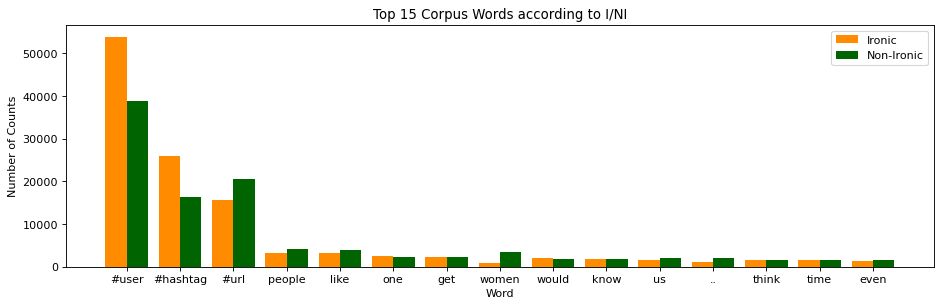
\includegraphics[width=\textwidth]{images/word_counts_i_ni.png}
    \caption{Bar plots for the top 20 most used words in the corpus according to the two classes.}
    \label{fig:bar_word_counts}
\end{figure*}

\subsection{Challenges of Data}

In manual irony annotation of tweets, \citeA{van2018exploring} found that among ironic tweets realized through polarity contrast (71\% of all ironic tweets), half were only identifiable as such by hashtag use. This means that absence of hashtags in the data will likely increase the difficulty of the task (see also \citeA{maynard2014hashtag} on hashtag-based classification). 

Another limitation of the dataset is the fact that we have no way of accessing conversational context for reply tweets, which has been shown to be significant for identifying irony \cite{joshi2015harnessing, wallace2015sparse}. Single tweets and reply tweets are treated the same in the dataset, even though we might expect that irony would function differently for them. 

\subsection{Data Pre-Processing}

% do we also remove the hashtag tags?
Our pre-processing methods are dependent on which features are being generated. However, for most features we remove the generic hashtag, user and URL tags from the tweets before processing them. These are then tokenized by the \emph{TweetTokenizer} provided by NLTK\footnote{\url{https://www.nltk.org/api/nltk.tokenize.casual.html}}. This is optimized to capture smileys and long words which are not standard English. 

\section{Features}
 We took a feature engineering approach to the task, as such approaches have yielded good results in the past (references) and have the benefit of being more interpretable than end-to-end embedding approaches. We explain how the features were generated and our hypotheses about how they might contribute to distinguishing ironic and non-ironic users. 
 
 We divide this section into two sub-sections, the first detailing the features used in the final model as in Fig.\ref{fig:model_representation}, and second describing the features we experimented with but decided against using as part of the final feature vector.
 
 \subsection{Model Features}
    \subsubsection{TR - Stylistic Features}
        Our first approach was centered around creating features that represent the profile's style. To do this, we perform simple counts on each author's output, which are then divided by the total number of tweets by the author (200 in this task). We generated the features displayed in Table \ref{tab:count-features}.
        \begin{table*}
            \centering
            \begin{tabular}{ l l } 
             \textbf{Avg. Vocab Size:} & Number of unique tokens per tweet \\
             \textbf{Avg. Token Number:}  & Number of tokens on average per tweet \\
             \textbf{Vocab/Token Ratio:}  & Number of Vocab divided by tokens\\
             \textbf{Avg. Tweet Length:} & Number of characters on average per tweet\\
             \textbf{Avg. HASHTAG Counts} & Number of HASHTAGs on average per tweet\\
             \textbf{Avg. USERTAG Counts} & Number of USERTAGs on average per tweet\\
             \textbf{Avg. URL Counts } & Number of URLs on average per tweet \\
             \textbf{Avg. Emoji Counts } & Number of Emojis on average per tweet\\
             \textbf{Avg. Capital/Lower Case Ratio} & Ratio between upper and lower case per tweet\\
            \end{tabular}
            \caption{Count features used in the final system}
            \label{tab:count-features}
        \end{table*}
        
        The intuition about these features is to portray some of the main trends between the user-profiles. \citeA{irony_detect_twitter} argue that due to character limit restraints ironic tweets might achieve their goal by creative use of fewer words. We also believe that ironic users might use shorter replies and abbreviations to express irony. Structural features have also been used before in similar tasks \cite{irony_detect_twitter}.
        All hashtags and twitter handles have been replaced by generic markers in our data,  but previous studies have found that hashtag use is connected to sarcasm \cite{van2018exploring}, so we believe these counts would still be relevant for this task \cite{sarcasm_detection}.
        
    \subsubsection{TR - LiX Score}
        LiX is a measurement of text complexity developed in Sweden (Bjõrgsen, 1968) that uses a combination of a word and sentence factors. LiX is calculated by the following formula: 
        $$ \text{LiX} = (\% N_{Long Words}) + (N_{words}/N_{sentence}) $$
        
        We have set the threshold for long words at $t=7$, following \citeA{lix_score}, and we count the number of sentences by using a regular expression to find punctuation followed by a space or a new line: 
         $$\verb'[ ]+[.;?!]|[.;?!][ ]+|[.;?!]\n'$$
         
         There might be a risk of underestimating the number of sentences, but the LiX statistics on our dataset: $\mu = 33.3; \sigma = 6.3; max=61.6; min=16.7$, correspond to a 7th grade lexical complexity, which seems adequate for a social media with a microblog format.
        
        Our intention with this metric, similar to the stylistic features, is to model that ironic profiles might use less complex structures to reach a wider audience and easier to understand tone.
 
        
    \subsubsection{TF-IDF}
        Words frequencies have been used to model sarcasm \cite{sarcasm_detection}, and it makes intuitive sense that the use of certain words might be indicative of irony. To model this problem, we attempted the Term-Frequency-Inverted-Document-Frequency (TF-IDF).
        
        TF-IDF is based on the intuition that tokens which are rare in a corpus might contain more information if they appear in a specific document. For this task, we implemented a parameter to allow switching between an author's whole output or a single tweet as a document. For the final feature vector, we used single tweets as documents and our entire training data as a corpus, as we found this improved performance relative to author documents.
        
        There are different approaches to TF-IDF when it comes to normalizing term frequency (TF). In our implementation, we use the $log_2$ scale, which means that eventually more counts contribute less and less.
        
        IDF is calculated by first creating an encoding vector, where each position corresponds to a term in the corpus. We  count in how many documents of the corpus each term occurs We then can calculate the \emph{idf} vector: $$idf=log_2(\frac{N}{n_t})$$ where $N$ is the number of document and $n_t$ is the number of documents where $t$ occurs. Note that we don't smooth out the  division, as we only consider terms which are present in the corpus. The term \emph{tf} is calculated by counting the number of terms which are present in the $idf$ vector of size $m$ for each tweet, and this is saved into a matrix of size $\text{documents} \times m$. We then want to ensure that terms are scaled to a logarithmic scale, and to do this we perform the following operation on the matrix:
        \begin{equation*}
            \begin{cases}
              0, \emph{}{tf}=0\\
              1+log_2(\emph{}{tf}), \emph{}{tf}>0\\
            \end{cases}
        \end{equation*}
        We then multiply each of the document vectors by the $idf$ to obtain the final \emph{tf-idf} vector for a specific author. In the case of using tweets as document, we obtain the average tweet \emph{tf-idf} vector for each author. For the profanity TF-IDF, we lowercase all the tweets and stem the words to match the same root, while for word TF-IDF we simply lowercase and remove any hashtags in the set.
        
    \subsubsection{POS Tags}
        To obtain POS tags we decided to use the \emph{Universal Part-of-Speech Tagset}, which is described in NLTK's documentation\footnote{\url{https://www.nltk.org/book/ch05.html#tab-universal-tagset}}. It consists of 12 different POS tags which are counted across each author, after tokenization and removal of tweeter tags, averaged to obtain the average POS counts for each author. Some parts of speech tag like ADVs and ADJs have been shown to be lexical markers for irony \cite{irony_detect_twitter}. We decided to drop the tags NOUN, X, PUNC, as they are already encoded in other features. Nouns tend to correlate strongly with token counts, punctuation we decided to create features to encode specific types of punctuation as described in (4.1.6) and X, representing words that the model couldn't assign a POS to, are usually few and not relevant for classification.
        
    
    \subsubsection{Profanity}
    
    
    Some of the earliest work on irony detection \cite{burfoot2009automatic} used the presence of profanity as a feature to identify irony in news headlines, and research has since shown that online communities use profanity in different ways and could be used to distinguish them \cite{wang2014cursing}. Therefore we hypothesized that profanity use might also be different for ironic and non-ironic users, for example in the frequency and types of words used. 
    
    We implemented this feature based on a profanity list on GitHub\footnote{\url{https://github.com/zacanger/profane-words}} with 2864 words. We created count vectors for the Twitter users and reduced dimensionality via PCA to 14 principal components. The data was pre-processed with tokenizing and stemming before creating the count vectors, as our profanity list only contained lemmas. 
    
    This feature obviously overlaps with TF-IDF, which also counts profanity along with all other words, but we hoped that isolating this lexical group might help us find patterns that would otherwise be lost in the TF-IDF features. 
    

    \subsubsection{Sentiment Analysis}
        Irony can be used to attribute a sentiment value towards a specific target \cite{irony_detect_twitter}, and so we would imagine that this would also be a feature that helps distinguish an Ironic user from Not-Ironic one.
        For this feature we used the framework \emph{VADER-Sentiment-Analysis}\footnote{\url{https://github.com/cjhutto/vaderSentiment}}, which is a lexicon and rule based sentiment analysis tool which returns 4 features: \emph{positive}, \emph{negative}, \emph{neutral} and \emph{compound} values. The latter is a combination of all previous 3. 
        
        Initially, we attempted to model the sentiment by calculating a metric which would attempt to count the number of sentences which would have high polarity in sentiment (high values in both positive and negative sentiment). However, this method seem to filter out too much information and the results weren't too promising.
        
        For this reason, we decided to instead calculate sentiment for each tweet and proceed to combine them using statistical methods. We attempted both the average vector across all tweets \textbf{(M)} as well as the standard deviation \textbf{(SD)} for each metric. From our experimentation, the latter seemed to perform better, and we speculate it is due to the fact it captures information about how a user usually tend to deviate from his average expression. 
        
    \subsubsection{Punctuation}
    We also included punctuation as a feature. These are features often used for irony detection as in \cite{Pathways_punct}. We separated each type of common multiple punctuation such as \textbf{!!!}, \textbf{???} and \textbf{...} as well as \textbf{quotation marks} and single punctuation. They were expected to be used differently in ironic versus non-ironic text. We filtered these patterns by using the the python regular expression library re \footnote{\href{https://docs.python.org/3/library/re.html}{RegEx}}. In the end we worked with the average number of punctuation per tweet for each user.
    
    
\subsection{Unused features}

%misspellings 
%embeddings
%syntactic complexity (with parsing and dependency trees)


    \subsubsection{Word Embedding}
        We also experimented with word embeddings as our model did not have any features that would encode context or semantic meaning of words. We assume that the semantics of certain words might be important to discern irony, namely when synonyms/antonyms are used to express a certain opinion.
        We experimented with the word-embeddings provided by \emph{Gensim}\footnote{\url{https://github.com/RaRe-Technologies/gensim-data}}. These are GloVe embeddings trained on a twitter corpus and we tested with different embedding sizes ($n \in {25.50.100})$.
        
        With the model, we average the embeddings for each word in an authors tweet to represent it by it's average embedding. We collect all of these representations for each of the authors tweets and then average them to collect the final embedding vector for the author.
        
        We then concatenate this vector with the other features to be used by the classifier. The results we obtained using these embeddings resulted in a generally worse performance when performing cross validation. We also tested these features in isolation, and we could see that it did achieve about $80\%$ accuracy, but when combined with the other features it didn't help the classifiers.
      \begin{figure*}[!h]
        \centering
        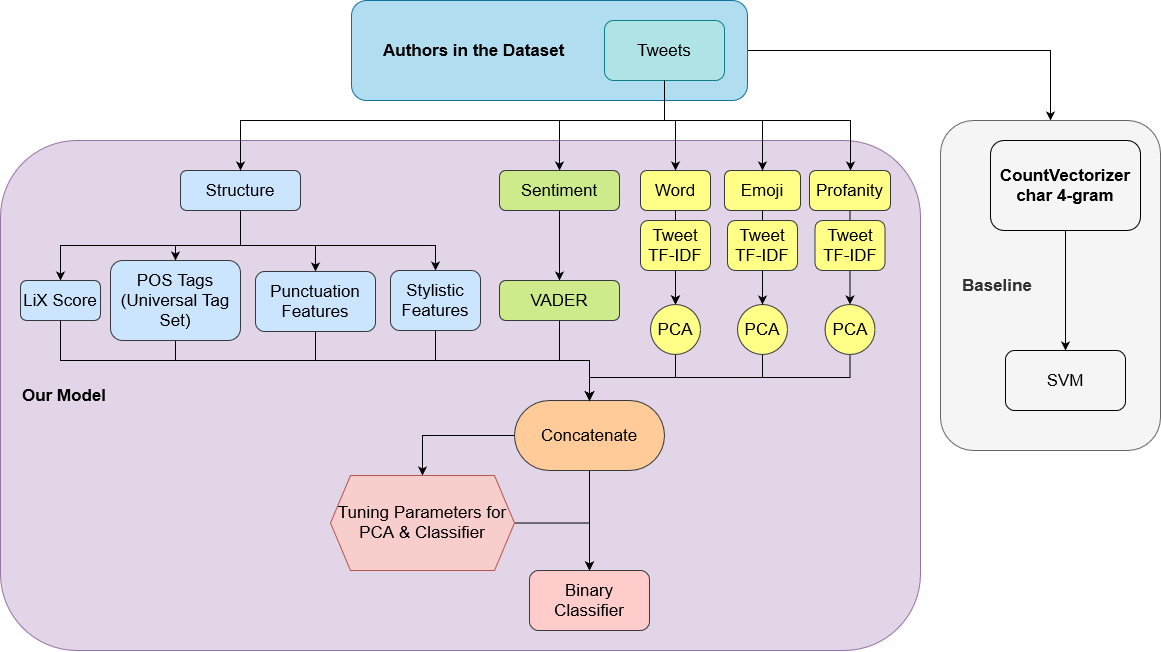
\includegraphics[width = \textwidth]{images/lang_proc.png}
        \caption{Final Model Used and Baseline Model representation}
        \label{fig:model_representation}
    \end{figure*}      
     \subsubsection{Misspelling}
    
    We thought that misspelling might be a good indicator of irony. By using PySpellchecker \footnote{\href{https://pyspellchecker.readthedocs.io/en/latest/}{PySpellchecker}} we found the misspelled words and set them in relation to the total number of words. However, it seems that the results greatly overlap for both classes and it is not a very practical feature for the classification. Because the misspellings did not add significant information, we did not use this feature out for our model training. We suspect that misspellings are in general very common on social media.
    % Use cross validation with the permutation_importance to average out the importance of different features
    % This is because different splits cause different features to be less or more important. 
    
    
    \subsubsection{Syntactic Complexity}
    
    Another type of feature we considered was syntactic complexity, which we hypothesized could be higher for non-ironic users.
    
    Syntactic complexity can be estimated in a number of ways including NP density, tree height and the number of high-level constituents per sentence \cite{barnwal2017using}. All of these approaches require parsing, which we did with \verb'spacy''s Dependency Parser\footnote{\url{https://spacy.io/usage/linguistic-features#dependency-parse}}. We tried implementing tree height, but the process proved very slow and expensive, and we dropped the feature so we could keep our model lightweight. We incorporate some syntactic information with POS counts, so it is not totally absent from our model.


\section{Methods}
    % Split the Train into 70% train and 30% test, and we do cross validation to 
    % - Tune parameters (PCA)
    % - STD / mean in Sentiment (etc)
    % Test on the 30% which the model hasn't seen to estimate performance.
    % Show cross validation results

\subsection{Baseline}
    In the task-webpage \cite{irony_detect_twitter}, the suggested baseline indicated was a char or word gram model, followed by the SVM. We followed this recommendation to create our own baseline, by using the \emph{CountVectorizer} class and the SVM as implemented by SKLearn. We experimented with different $n$, using cross-validation and found that a 4-char model worked best. This will be used in our results as the baseline for this task.

\subsection{Experiments}
    For all our classifiers and different features we followed the methodology of creating a $70-30$ split of the training data, where $70\%$ of the data was used for training/cross-validation and the last $30\%$ were used to test the classifiers. 
    
    To select different features, we would start by using them in isolation with the different classifiers and see the results on the cross-validation. If the accuracy was $>70\%$ then the features would be considered to be concatenated to the final feature vector.
    The features that weren't included often meant that the models would perform worse if they were added. 
    
    We also considered different dimensional reduction methods, namely \verb'PCA' and \verb'SparsePCA' for the TF-IDF vectors due to their large dimensions. It is also desirable that the final vector is somewhat interpretable, so we only applied these to the TF-IDF vectors, by far the largest dimensional features in our model. \verb'PCA' was cheaper and the results were comparable to \verb'SparsePCA' so this was used as our reduction method.
    
    We found the best performing \verb'PCA' dimensions for each of feature by performing a grid-search with cross-validation on the training data and the values found were $\text{emoji-PCA}_n = 4$, $\text{profanity-PCA}_n = 14$, $\text{word-PCA}_n = 20$. These results make intuitive sense, where the dimensions increase in terms of complexity of the features and their importance for the final classification. 
    
    In terms of classifiers, we used 4 different methods: \textbf{random forest} (\verb'RandomForestClassifier'), \textbf{support vector machines (SVM)} (\verb'svm.SVC(gamma="auto")'), \textbf{logistic regression} (\verb'LogisticRegression') and \textbf{nearest neighbour (NN)} (\verb'KNeighborsClassifier') for our task. All classifiers with the exception of Random Forests are sensitive to highly different scaled values, so we normalize all features using the \verb'StandardScaler', which subtracts the mean and divides by standard deviation, from \verb'SKLearn'. When doing cross-validation, we always reported the values for each of these classifiers and we could see that each feature tended to impact them in different ways.
    
    The \emph{RandomForestClassifier} is the best performing across all metrics and features. For this reason, we attempted to do parameter tuning for this particular model. We did this by using grid-search, but found no parameters which performed better than those provided by SKLearn, so the parameters were left unchanged.
    
    We present results for both the Cross-Validation and Test splits. For test, we chose the models which performed the best in the Cross-Validation. The final model we use is displayed in fig. \ref{fig:model_representation}. We also report the performance of our best classifier (Random Forests) on the task test set.
    


\section{Results}
We find that all classifiers except NN perform better than the baseline in both cross validation and on the test data we separated from the training data. \par

\begin{table*}[!h]
    %\captionsetup{font=footnotesize}
    %\footnotesize
    \centering
    %\rowcolors{1}{}{white}
    \begin{tabular}{ll|ll}
    \toprule
      & \textbf{Train} & \textbf{Test} &  \\
      \textbf{Classifier} & \textbf{Accuracy (\%)} & \textbf{Accuracy (\%)}  & \textbf{F1-Score (\%)}  \\
    \midrule
    (SD) Random Forest & \textbf{100} & \textbf{91.84} & \textbf{91.83} \\
    (SD) Log. Reg. & 97.51 & 89.79 & 89.83 \\
    (SD) SVM & 97.22 & 89.12 & 89.12 \\
    (SD) 1-NN & \textbf{100} & 81.97 & 82.01 \\
    (SD) 3-NN & 92.23 & 87.76 & 87.79\\
    (SD) 5-NN & 88.83 & 82.65 & 85.71\\
    (M) Random Forest & \textbf{100} & 91.50 & 91.49 \\
    (M) SVM & 97.00 & 88.78 & 88.78 \\
    (M) Log. Reg. & 97.78 & 90.14 & 90.16 \\
    
    \hline
    Baseline (2-Char) & 85.09 & 82.65 & 82.39 \\
    Baseline (3-Char) & 87.24 & 83.67 & 83.60 \\
    Baseline (4-Char) & 87.24 & 84.35 & 84.36 \\
    Baseline (5-Char) & 88.89 & 82.65 & 82.70 \\
    \bottomrule
    \end{tabular}
   \caption{Cross-Validation on 70\% of the train data, n splits = 7. In bold, the best performing metrics. (M) denotes that the mean sentiment was used to combine the Tweet Sentiment, while (SD) denotes standard deviation was used.}
    \label{tab:cross_validation_results}
\end{table*}


Our results show that only the 1-NN models does not outperform the baseline, tab. \ref{tab:cross_validation_results}. The best baseline model (4-Char) performs with an accuracy of 87.24\% on the training set and on the test set with an accuracy of \textbf{84.35\%}, an F1-score \textbf{84.36\%}. We see that the random forest classifier obtains the best results. It performs with 100\% accuracy on the train data and \textbf{91.84\%} accuracy with and a F1-Score of \textbf{91.83\%} during cross validation using standard deviation on the sentiment across a users tweets. The scores using the mean sentiment (M) per a users tweet performs a little lower on the test set but still over 91\%. The other models do not perform as well. Logistic regression and SVM still outperform the baseline models with over 89\% in both accuracy and F1-Score.

Our models also outperform the best baseline when we trained on 70\% of the provided training data and tested on the remaining 30\%. The baseline model performs with an accuracy of \textbf{84.92\%} and an F1-score of \textbf{84.96\%}, see tab. \ref{tab:test_results}. All classifiers using our features, random forest, logistic regression, and SVM, outperform the baseline both using sentiment mean and SD. The best performing classifier is again random forest using SD for the sentiment with an accuracy and F1-score of \textbf{96.03\%} and \textbf{96.04\%} respectively. The same classifier using mean sentiment is close behind. Both logistic regression and SVM achieve accuracies and F1-scores above 90\%. Random forest is the best performing classifier in all cases. \par

The results for the \textbf{tasks test dataset was an accuracy of 95.56\% }, using the Random Forest and averaging the sentiments in tweets with VADER [(M) Random Forest]. These results are similar to the performance of the same classifier on our 70/30 split of the training data (acc: 95.24\%, see tab. \ref{tab:test_results}). 

It seems that the performance on the 30\% is a good indicator for performance on the official test set.

\subsection{Feature Importance}\label{sec:feature_imp}
We also discovered that not all features have the same importance, and that there are differences in their importance between classifiers. For that we used \verb'permutation_importance' from \verb'sklearn.inspection' \footnote{\url{https://scikit-learn.org/stable/modules/permutation\_importance.html}} to calculate the importance of each feature. This method calculates the influence of each feature has by comparing the original accuracy score with the score of obtained if different features are removed.  \par

With the permutation importance we can see the importance of each feature for each classifier. For random forest \verb'avg_user_hashtag_count' and \verb'auth_vocabsize' seem to be the most important. While the other features have noticeable less influence, figure \ref{fig:fi_rf}. 1-NN is even more extreme. Here only \verb'avg_tweet_length' and \verb'LixScore' seem to be important, figure \ref{fig:fi_1NN}. Both logistic regression and SVM have the highest importance for \verb'word_pca11', \verb'auth_vocabsize' and \verb'qu' (average number of question marks), figure \ref{fig:fi_logreg} and \ref{fig:fi_svm}. For these classifiers, the importance of features are also more equally distributed than for the other classifiers especially 1-NN. We see that different features are more important than others for different classifiers and that logistic regression and SVM have generally a higher feature importance for each feature.


\begin{table}[h]
    %\captionsetup{font=footnotesize}
    %\footnotesize
    \centering
    \small
    %\rowcolors{1}{}{white}
    \begin{tabular}{l|ll}
    \toprule
    \textbf{Classifier} & \textbf{Accuracy (\%)}  & \textbf{F1-Score (\%)}  \\
    \midrule
    (SD) Random Forest & \textbf{96.03} & \textbf{96.04} \\
    (SD) Log. Reg. & 90.47  & 90.49 \\
    (SD) SVM & 92.06 & 92.08 \\
    (M) Random Forest & 95.24 & 95.25 \\
    (M) Log. Reg. & 90.47  & 90.50 \\
    (M) SVM & 92.06 & 92.08 \\
    \hline
    Baseline (4-Char) & 84.92 & 84.96 \\ 
    \bottomrule
    \end{tabular}
   \caption{Test results on the remaining 30\% of the data. The baseline model is a 4-gram char BOW model followed by a SVM for classification. In bold, the best performing metrics.}
    \label{tab:test_results}
\end{table}



\section{Discussion}
% Analyse where the network misclassified (some examples) 
%remember we classify authors not tweets -> example would be author level
% Features that contribute the most (#hashtag) is usually used a denotation of irony. Vocab size (smaller for I), usually simple language. 
% Limitations: Context, while we attempted a simple embedding usage, our model currently has no context information.
% - While we avoided deep methods to allow for more interpretable features, the fact that half our points are resulting from PCA  means that it's not clear what some features are. 
% Our model might need some modifications to scale (namely the TF-IDF) as more data would require much more space to store the vectors. Clipping vocab could be used, stemming.
% Refer that due to the lack of tweet level labels it~s hard
% Considering different models learned through different features we could consider using an ensamble (merging probabilities of different models for different features).
% Author VS Tweet level and sample size. (How data is anotaded)
\subsection{Model Performance}

Our results show that the classifiers SVM, logistic regression and especially random forest perform very well with our features. Of the NN-classifiers, 3-NN performs best, but still lags a couple of percentage points behind the better-performing models. Our highest F1-score with random forest is 96.04, an F1-score that according to \citeA{sarcasm_detection}'s survey of the field is only topped by \citeA{ghosh2015sarcastic}, who obtain a score of 97.5 with a distributional semantics approach. 

Such high results are rather surprising considering the relative simplicity of the features used in our model. Especially the lack of semantic similarity or incongruity features (although perhaps sentiment SD could be interpreted as such), which are otherwise widely used \cite{reyes2012humor, riloff2013sarcasm, joshi2015harnessing, joshi2016word}, makes this a remarkable result.

However, considering that a simple char-gram model paired with SVM is able to obtain an F1 of 84.36, we suspect that this dataset is simply easier to classify than previous datasets in similar tasks. This might have to do with how this dataset was annotated and how the Twitter users were sampled. Unfortunately the task authors do not provide us with this information, so it's unclear what makes this dataset unusual. However, we do know that some ways of collecting twitter data, for example based on \#irony hashtags, can create datasets that are easier to classify \cite{sarcasm_detection}, so data collection and sampling methods likely play role here as well.

Unlike most previous research that focuses on the tweet-level irony detection \cite{sarcasm_detection}, we are classifying irony on the user level. This is significant, as previous research \cite{cyberbullying} shows that the majority of hate speech is produced by a small minority of people. It might therefore be more effective to identify hateful/sarcastic users than individual utterances. It might also be the case that identifying irony on the user level (both in terms of annotation and prediction) is more robust than doing so for individual tweets, and that this is partly responsible for the high F1-score. 

As seen in Table \ref{tab:test_results} the high scores were robust (and even improved) when only 70\% of the data was used for training. 

\begin{figure}[!h]
    \centering
    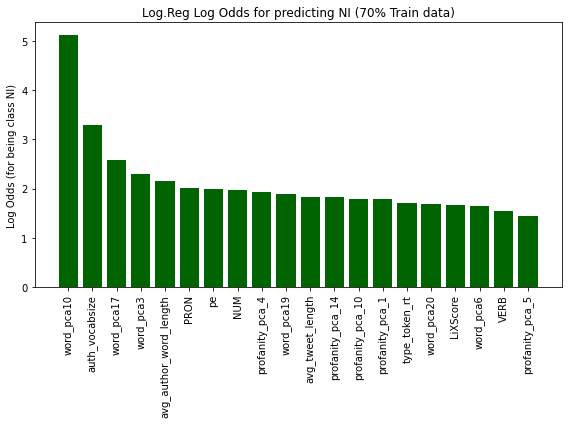
\includegraphics[width=0.48\textwidth]{images/NI_features_log_reg_odds.png}
    \caption{Log odds for predicting NI}
    \label{fig:ni_log_odds}
\end{figure}

\begin{figure}[!h]
    \centering
    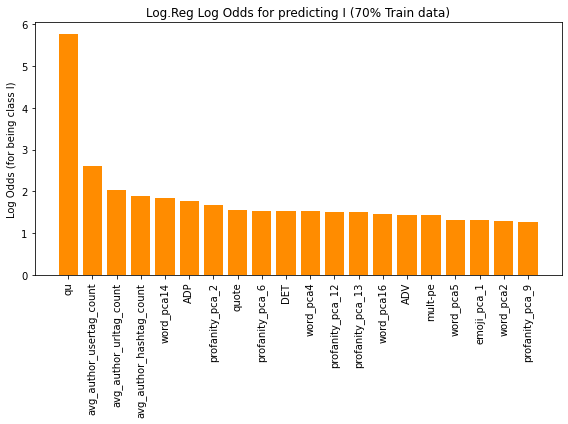
\includegraphics[width=0.48\textwidth]{images/I_features_log_reg_odds.png}
    \caption{Log odds for predicting I}
    \label{fig:i_log_odds}
\end{figure}

\subsection{Feature Peformance}

While developing our different features we found that even the stylistic count features on their own performed similar (about 80\% accuracy) to the Baseline model, despite being quite primitive. This means that simply by looking at the general stylistic characteristics of an author a machine learning model is able to separate the two classes. This indicates that the difference between ironic and non-ironic tweeting styles really is very distinct on the user level. Every other feature yielded small improvements, with TF-IDF being the highest contributor. 



Based on feature permutation (see Appendix), we found that vocabulary size, hashtag counts and question marks were among the most significant features, as well as some TF-IDF PCA vectors, i.e. stylistic and lexical features. This is consistent with previous studies \cite{gonzalez2011identifying, joshi2015harnessing} where lexical features (especially unigrams) are used a baseline and core of more complex models. Studies that find strong effects of punctuation and similar stylistic features include \citeA{bouazizi2015sarcasm} and \citeA{van2018exploring}. Per Table \ref{tab:cross_validation_results}, using the sentiment standard deviation rather than the mean also generally improved results by a small amount. The standard deviation might be better than the mean at capturing incongruencies in polarity, which are often indicative of irony. 

For a more fine-grained analysis, we find the log odds for predicting ironic and non-ironic users in Figure 3 and 4, respectively. We see that ironic users are characterized by a higher use of question marks, more URLs, usertags (replies) and hashtags, while non-ironic users have a larger vocabulary size and word length, among others. Some PCA features also increase the odds of being non-ironic, which again might be related to the larger vocabulary of those users.

While looking into the values of different words in the TF-IDF, we noticed that sometimes words specific to a single user, as for instance a promotion code, will have very high values in the TF-IDF vector, as they fit the criteria of being used by only a single user multiple times. For instance, in \verb'word_pca_10' when trained on 70\% of the data, if we softmax the weights on that PCA component and sort them according to their scores we find the following words score highest: `women', `:', `and', `men', `calm',  `gay', `guard', `code', `USER-PROMO-CODE'. As we can see, some words here might be related with irony and stereotypes, like `gay' and `women', but the user promotional code is not related at all to the task and might add noise. To ensure a better quality of these features, we could have opted for stemming and removing stop words or words that only appear in a single user (to capture cases like promotional posts), while accepting that we might lose some information.

%An observation furthered by the good performance of the baseline which is only based on char grams. It is interesting to see how these few relatively simple features can already lead to results as good.
% While we aimed to use classical machine learning methods paired with easy to understand features to discern patterns between the two classes, we still were in need of using PCA to reduce the dimensions of the large resulting TF-IDF vectors from this dataset. This means that a lot of the information provided by the PCA is not easy to interpret. We expect the resulting vectors to contain features that are used a lot in a few tweets and that vary a lot between different authors. 

% We used classical ML for explainable results. A analysis of each feature could give us an approximation about what an ironic style is. However, the majority of our features are based on PCA which reduces the explainability again as it is not necessarily clear what these features mean.

%author level 
Due to the nature of the task as an author classification task we cannot say if a particular tweet is ironic. Instead we are only able to classify by all their tweets, but not exactly point out where irony or stereotypes are present. However given the annotations for the dataset, one would have to identify specific cases of irony/stereotypes manually to allow for this type of classification. It is also not clear how many ironic tweets make a user an irony-spreader or not. Therefor is unclear how the system would perform in the wild or for larger datasets, when the annotation is not as clear or generated in other ways. 
 
\subsection{Limitations}

Our model has several limitations and areas for improvement. A general drawback is the time it takes to generate the features for the training and test data, particularly for the TF-IDF and profanity PCA features. This means the model would not scale well in terms of time and space usage. To avoid this scalability problem the number of terms for TF-IDF could be reduced by clipping the vocabulary or stemming the words in each tweet and accepting some information loss in exchange for a faster performing system.

Currently our model does not consider context. Our features at most capture a unigram language model by the usage of TF-IDF, but even then it's distorted by PCA. While we attempted embeddings, these were not beneficial to the task. This is a bit surprising considering the success others have had with word embedding-based features in conventional ML \cite{joshi2016word}. Word embeddings in isolation might not capture enough information, and would need to be processed in some way before being used in the model. They would also likely be more useful in a deep-learning approach, which is the type of model in which they are usually used \cite{zhang2019irony, sarcasm_detection}.

That being said, we believe our model would require features that encode semantic and pragmatic information, incongruencies or even ontologies to interpret if some words are being used out of the expected context

Another direction for future work relates to the fact that the different classifiers appear to rely on different features (see Appendix). Considering this, an ensemble method could be used to combine different classifiers to optimally use more of the features. We could for instance have a model that focuses on more low-level features, which word combinations are more likely, and a model like ours which uses more high-level and general features. 

% Mistakes:
% Probabilities are: I / NI
% c75bc1b6dd7d283e1ff17a2a8a512a76.xml : 0.09 / 0.91 (Correct label I) ⛔
% a7e7cc1908ee78179a883a47ae68c52f.xml : 0.5 / 0.5 (Correct label NI), Essentially this one was random ⛔
% e19408d8b77473ec2c23d11bd589e2fe.xml : 0.01 / 0.99 (Correct label I) ⛔The worst mistake
% ce6df51b12f065042c81f98ed0773687.xml : 0.49 / 0.51 (Correct label I) ⛔
% ceec7ed40f2ddeebd501ba2b785ff305.xml : 0.47 / 0.53 (Correct label I) ⛔
% 8ee99a8ea76169ee47b978f6cce69fb0.xml : 0.48 / 0.52 (Correct label I) ⛔
% 446a550e12709539e1af83c2dba75de7.xml : 0.01 / 0.99 (Correct label NI)✅
% 53405c12b5e86d2f3847850939d712b0.xml : 0.04 / 0.96 Correct Label (NI)✅
% 14c6666bf57dc5b6f5334ed8a65bffd4.xml : 0.97 / 0.03 Correct Label (I)✅

% Interesting find: "We don't buy bitcoin We earn bitcoin From Mining I'm ready to show 10 lucky people how to earn 0.1BTC" is repeated accross 5 users - what is this?



\section{Conclusion}
We tackled the challenge of detecting irony and stereotype spreaders by focusing on creating stylistic and lexical features. We compared the performance of our features with the suggest baseline for the task, a 4-char gram model followed by an SVM, with our own features. Our features combined with a random forest classifier outperform the baseline by $\approx 11\%$ on a $30\%$ split of the training data. We also obtained $95.56\%$ accuracy on the task's test set, by using a random forest classifier with our features. We can see room for improvement to focus on identifying passages for irony and sarcasm usage and develop features which focus on encoding context and semantic relationship between words. 

\bibliographystyle{apacite}
\bibliography{source}

\clearpage
\onecolumn
\section*{Appendix}\label{sec:appendix}

\begin{figure}[!h]
    \centering
    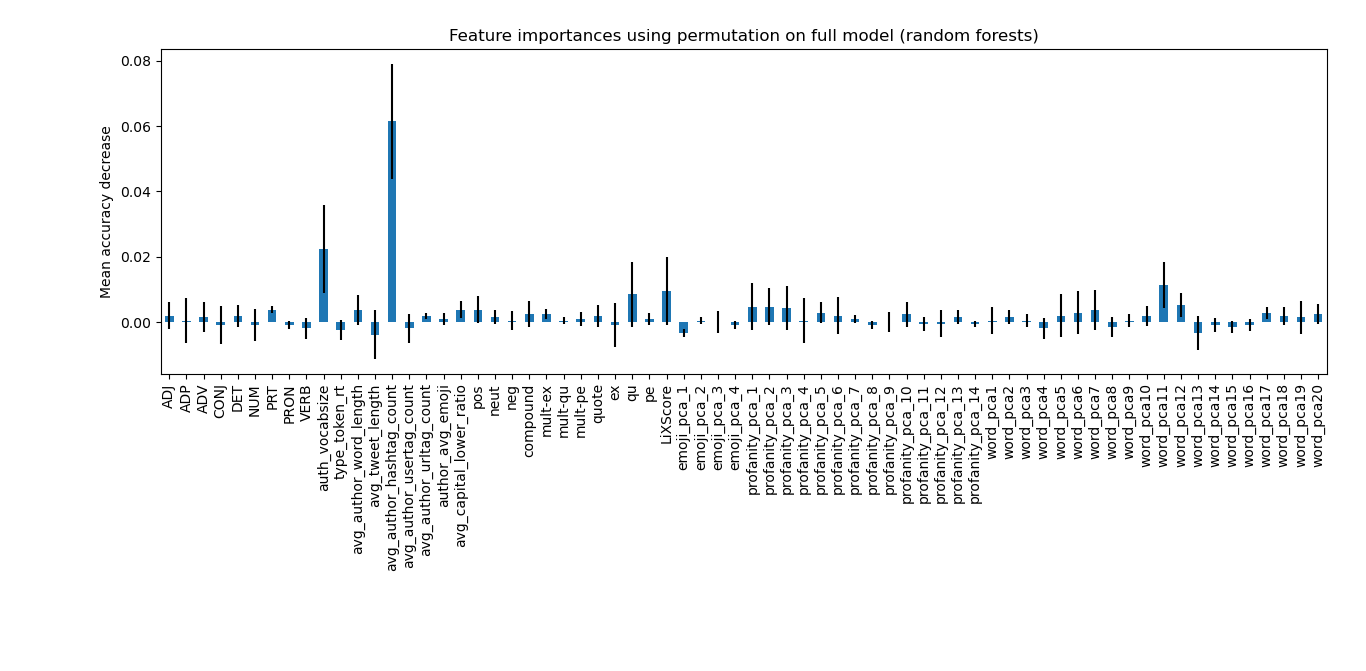
\includegraphics[width = \textwidth]{images/feature_importance_rf.png}
    \caption{Feature permutation for random forest regression}
    \label{fig:fi_rf}
\end{figure}

\vspace{0.1cm}

\begin{figure}[!h]
         \centering
         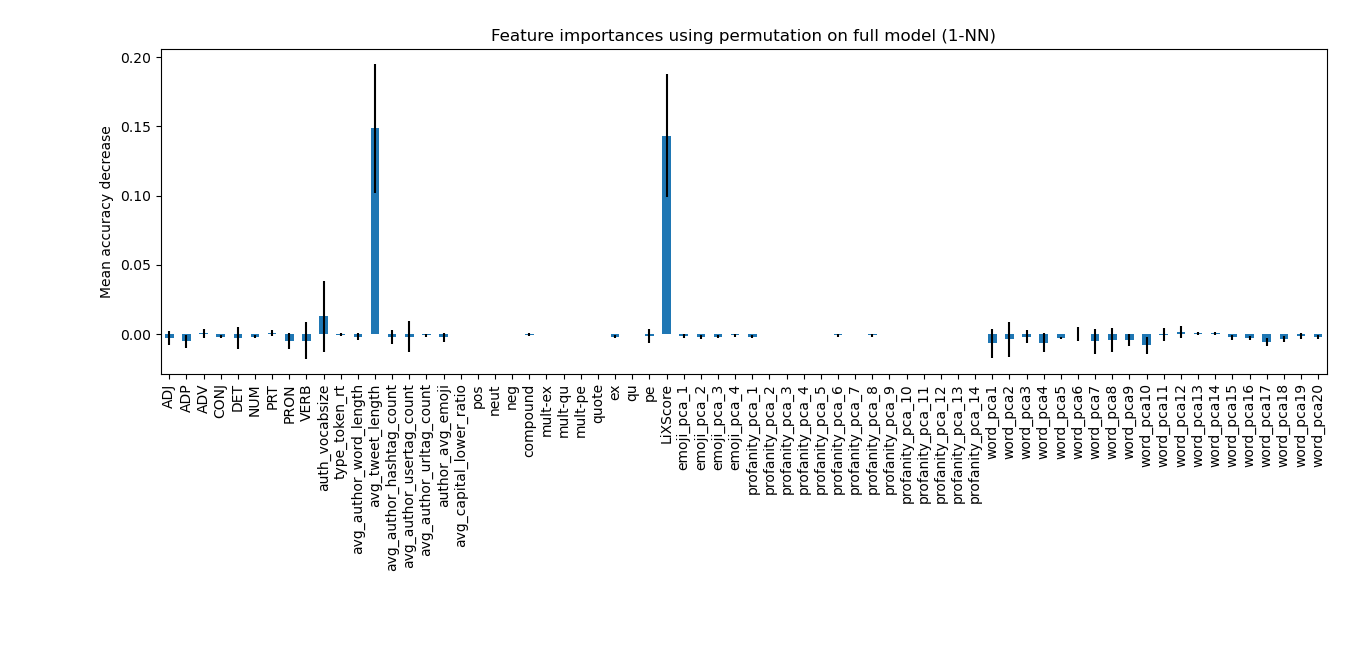
\includegraphics[width=\textwidth]{images/feature_importance_1NN.png}
         \caption{Feature permutation for 1-NN}
         \label{fig:fi_1NN}
\end{figure}

\vspace{0.1cm}

\begin{figure}
         \centering
         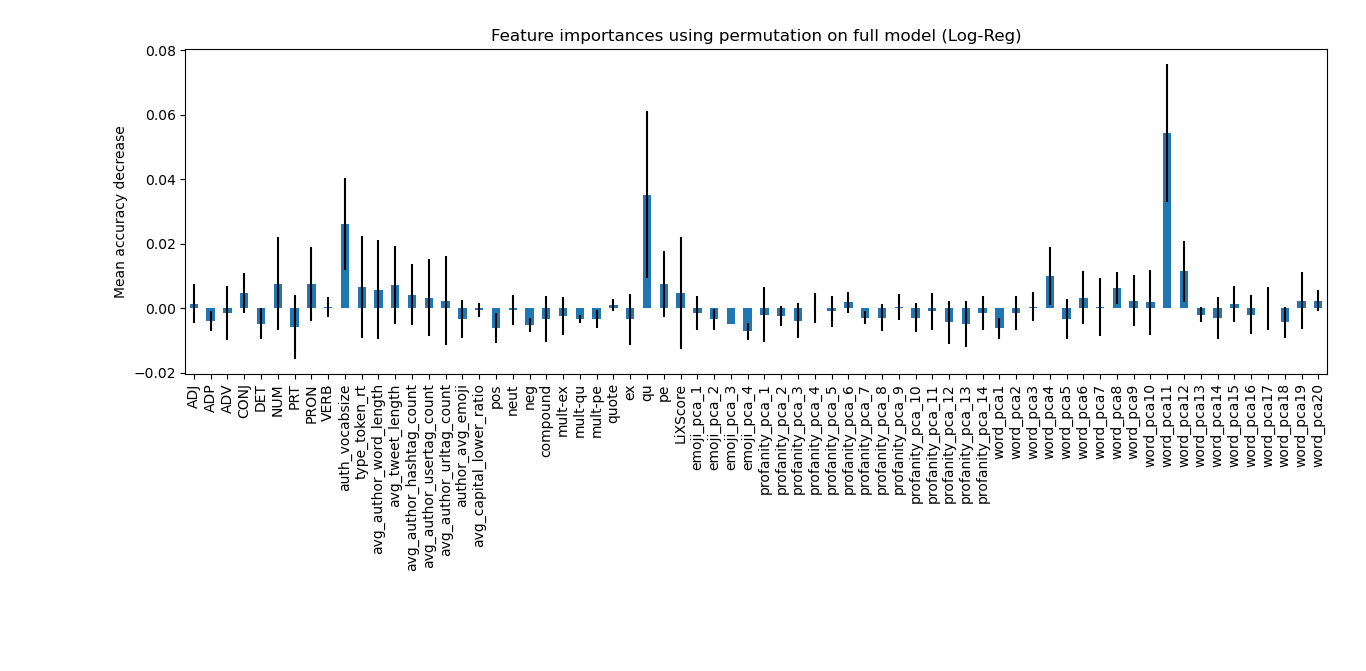
\includegraphics[width=\textwidth]{images/feature_importance_logreg.png}
         \caption{Feature permutation for Logistic Regression}
         \label{fig:fi_logreg}
     \end{figure}
     
\vspace{0.1cm}

\begin{figure}
         \centering
         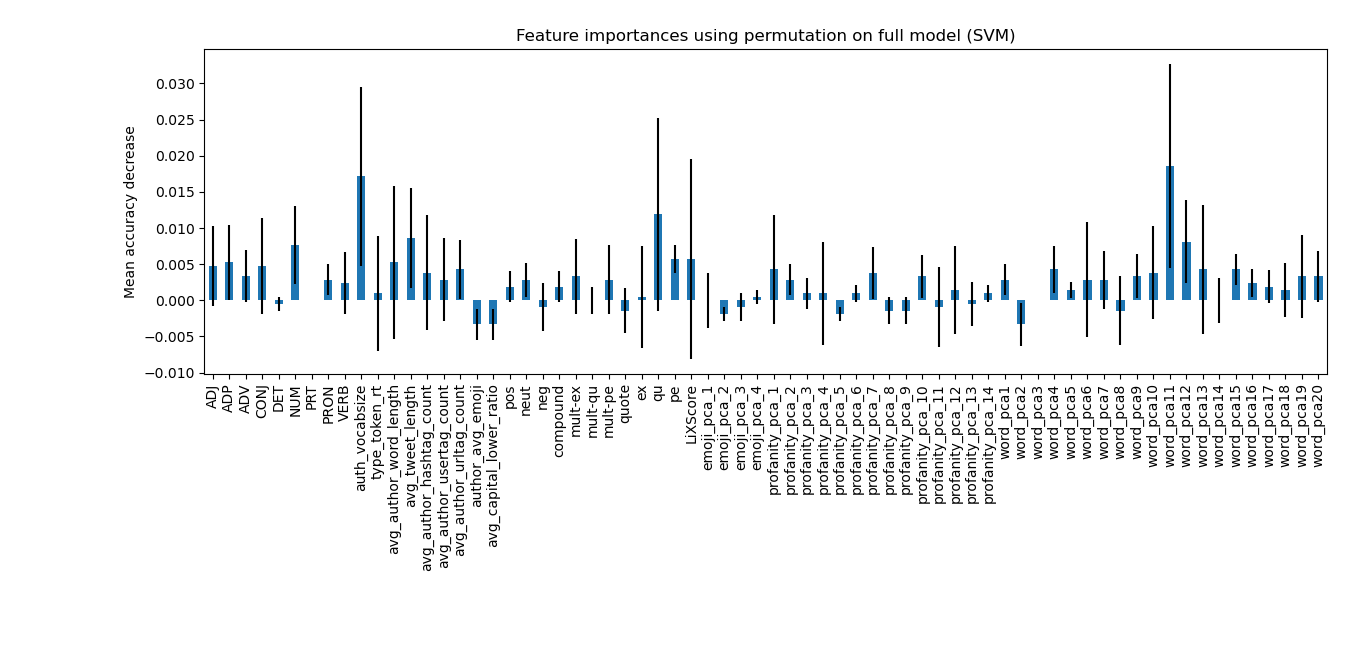
\includegraphics[width=\textwidth]{images/feature_importance_SVM.png}
         \caption{Feature permutatoin for SVM}
         \label{fig:fi_svm}
     \end{figure}

\end{document}